% GNUPLOT: LaTeX picture with Postscript
\begingroup
  \makeatletter
  \providecommand\color[2][]{%
    \GenericError{(gnuplot) \space\space\space\@spaces}{%
      Package color not loaded in conjunction with
      terminal option `colourtext'%
    }{See the gnuplot documentation for explanation.%
    }{Either use 'blacktext' in gnuplot or load the package
      color.sty in LaTeX.}%
    \renewcommand\color[2][]{}%
  }%
  \providecommand\includegraphics[2][]{%
    \GenericError{(gnuplot) \space\space\space\@spaces}{%
      Package graphicx or graphics not loaded%
    }{See the gnuplot documentation for explanation.%
    }{The gnuplot epslatex terminal needs graphicx.sty or graphics.sty.}%
    \renewcommand\includegraphics[2][]{}%
  }%
  \providecommand\rotatebox[2]{#2}%
  \@ifundefined{ifGPcolor}{%
    \newif\ifGPcolor
    \GPcolortrue
  }{}%
  \@ifundefined{ifGPblacktext}{%
    \newif\ifGPblacktext
    \GPblacktexttrue
  }{}%
  % define a \g@addto@macro without @ in the name:
  \let\gplgaddtomacro\g@addto@macro
  % define empty templates for all commands taking text:
  \gdef\gplbacktext{}%
  \gdef\gplfronttext{}%
  \makeatother
  \ifGPblacktext
    % no textcolor at all
    \def\colorrgb#1{}%
    \def\colorgray#1{}%
  \else
    % gray or color?
    \ifGPcolor
      \def\colorrgb#1{\color[rgb]{#1}}%
      \def\colorgray#1{\color[gray]{#1}}%
      \expandafter\def\csname LTw\endcsname{\color{white}}%
      \expandafter\def\csname LTb\endcsname{\color{black}}%
      \expandafter\def\csname LTa\endcsname{\color{black}}%
      \expandafter\def\csname LT0\endcsname{\color[rgb]{1,0,0}}%
      \expandafter\def\csname LT1\endcsname{\color[rgb]{0,1,0}}%
      \expandafter\def\csname LT2\endcsname{\color[rgb]{0,0,1}}%
      \expandafter\def\csname LT3\endcsname{\color[rgb]{1,0,1}}%
      \expandafter\def\csname LT4\endcsname{\color[rgb]{0,1,1}}%
      \expandafter\def\csname LT5\endcsname{\color[rgb]{1,1,0}}%
      \expandafter\def\csname LT6\endcsname{\color[rgb]{0,0,0}}%
      \expandafter\def\csname LT7\endcsname{\color[rgb]{1,0.3,0}}%
      \expandafter\def\csname LT8\endcsname{\color[rgb]{0.5,0.5,0.5}}%
    \else
      % gray
      \def\colorrgb#1{\color{black}}%
      \def\colorgray#1{\color[gray]{#1}}%
      \expandafter\def\csname LTw\endcsname{\color{white}}%
      \expandafter\def\csname LTb\endcsname{\color{black}}%
      \expandafter\def\csname LTa\endcsname{\color{black}}%
      \expandafter\def\csname LT0\endcsname{\color{black}}%
      \expandafter\def\csname LT1\endcsname{\color{black}}%
      \expandafter\def\csname LT2\endcsname{\color{black}}%
      \expandafter\def\csname LT3\endcsname{\color{black}}%
      \expandafter\def\csname LT4\endcsname{\color{black}}%
      \expandafter\def\csname LT5\endcsname{\color{black}}%
      \expandafter\def\csname LT6\endcsname{\color{black}}%
      \expandafter\def\csname LT7\endcsname{\color{black}}%
      \expandafter\def\csname LT8\endcsname{\color{black}}%
    \fi
  \fi
    \setlength{\unitlength}{0.0500bp}%
    \ifx\gptboxheight\undefined%
      \newlength{\gptboxheight}%
      \newlength{\gptboxwidth}%
      \newsavebox{\gptboxtext}%
    \fi%
    \setlength{\fboxrule}{0.5pt}%
    \setlength{\fboxsep}{1pt}%
\begin{picture}(7920.00,6800.00)%
    \gplgaddtomacro\gplbacktext{%
      \csname LTb\endcsname%
      \put(997,4735){\makebox(0,0)[r]{\strut{}$10^{-2}$}}%
      \csname LTb\endcsname%
      \put(997,5075){\makebox(0,0)[r]{\strut{}$10^{-1}$}}%
      \csname LTb\endcsname%
      \put(997,5415){\makebox(0,0)[r]{\strut{}$10^{0}$}}%
      \csname LTb\endcsname%
      \put(997,5755){\makebox(0,0)[r]{\strut{}$10^{1}$}}%
      \csname LTb\endcsname%
      \put(997,6096){\makebox(0,0)[r]{\strut{}$10^{2}$}}%
      \csname LTb\endcsname%
      \put(997,6436){\makebox(0,0)[r]{\strut{}$10^{3}$}}%
      \csname LTb\endcsname%
      \put(997,6776){\makebox(0,0)[r]{\strut{}$10^{4}$}}%
      \csname LTb\endcsname%
      \put(1099,4556){\makebox(0,0){\strut{} }}%
      \csname LTb\endcsname%
      \put(2137,4556){\makebox(0,0){\strut{} }}%
      \csname LTb\endcsname%
      \put(3176,4556){\makebox(0,0){\strut{} }}%
      \csname LTb\endcsname%
      \put(4214,4556){\makebox(0,0){\strut{} }}%
      \csname LTb\endcsname%
      \put(5252,4556){\makebox(0,0){\strut{} }}%
      \csname LTb\endcsname%
      \put(6291,4556){\makebox(0,0){\strut{} }}%
      \csname LTb\endcsname%
      \put(7329,4556){\makebox(0,0){\strut{} }}%
      \csname LTb\endcsname%
      \put(7431,4735){\makebox(0,0)[l]{\strut{} }}%
      \csname LTb\endcsname%
      \put(7431,5075){\makebox(0,0)[l]{\strut{} }}%
      \csname LTb\endcsname%
      \put(7431,5415){\makebox(0,0)[l]{\strut{} }}%
      \csname LTb\endcsname%
      \put(7431,5756){\makebox(0,0)[l]{\strut{} }}%
      \csname LTb\endcsname%
      \put(7431,6096){\makebox(0,0)[l]{\strut{} }}%
      \csname LTb\endcsname%
      \put(7431,6436){\makebox(0,0)[l]{\strut{} }}%
      \csname LTb\endcsname%
      \put(7431,6776){\makebox(0,0)[l]{\strut{} }}%
    }%
    \gplgaddtomacro\gplfronttext{%
      \csname LTb\endcsname%
      \put(397,5755){\rotatebox{-270}{\makebox(0,0){\strut{}$k = 2$}}}%
      \csname LTb\endcsname%
      \put(2190,6565){\makebox(0,0)[l]{\strut{}Mult Gr w Blk Jac}}%
      \csname LTb\endcsname%
      \put(2190,6286){\makebox(0,0)[l]{\strut{}Add Swz w Coarse}}%
      \csname LTb\endcsname%
      \put(2190,6007){\makebox(0,0)[l]{\strut{}Mumps}}%
      \csname LTb\endcsname%
      \put(2190,5728){\makebox(0,0)[l]{\strut{}linear}}%
    }%
    \gplgaddtomacro\gplbacktext{%
      \csname LTb\endcsname%
      \put(997,2468){\makebox(0,0)[r]{\strut{}$10^{-2}$}}%
      \csname LTb\endcsname%
      \put(997,2808){\makebox(0,0)[r]{\strut{}$10^{-1}$}}%
      \csname LTb\endcsname%
      \put(997,3149){\makebox(0,0)[r]{\strut{}$10^{0}$}}%
      \csname LTb\endcsname%
      \put(997,3489){\makebox(0,0)[r]{\strut{}$10^{1}$}}%
      \csname LTb\endcsname%
      \put(997,3829){\makebox(0,0)[r]{\strut{}$10^{2}$}}%
      \csname LTb\endcsname%
      \put(997,4170){\makebox(0,0)[r]{\strut{}$10^{3}$}}%
      \csname LTb\endcsname%
      \put(997,4510){\makebox(0,0)[r]{\strut{}$10^{4}$}}%
      \csname LTb\endcsname%
      \put(1099,2289){\makebox(0,0){\strut{} }}%
      \csname LTb\endcsname%
      \put(2137,2289){\makebox(0,0){\strut{} }}%
      \csname LTb\endcsname%
      \put(3176,2289){\makebox(0,0){\strut{} }}%
      \csname LTb\endcsname%
      \put(4214,2289){\makebox(0,0){\strut{} }}%
      \csname LTb\endcsname%
      \put(5252,2289){\makebox(0,0){\strut{} }}%
      \csname LTb\endcsname%
      \put(6291,2289){\makebox(0,0){\strut{} }}%
      \csname LTb\endcsname%
      \put(7329,2289){\makebox(0,0){\strut{} }}%
      \csname LTb\endcsname%
      \put(7431,2468){\makebox(0,0)[l]{\strut{} }}%
      \csname LTb\endcsname%
      \put(7431,2808){\makebox(0,0)[l]{\strut{} }}%
      \csname LTb\endcsname%
      \put(7431,3149){\makebox(0,0)[l]{\strut{} }}%
      \csname LTb\endcsname%
      \put(7431,3489){\makebox(0,0)[l]{\strut{} }}%
      \csname LTb\endcsname%
      \put(7431,3829){\makebox(0,0)[l]{\strut{} }}%
      \csname LTb\endcsname%
      \put(7431,4170){\makebox(0,0)[l]{\strut{} }}%
      \csname LTb\endcsname%
      \put(7431,4510){\makebox(0,0)[l]{\strut{} }}%
      \csname LTb\endcsname%
      \put(1099,4689){\makebox(0,0){\strut{} }}%
      \csname LTb\endcsname%
      \put(2137,4689){\makebox(0,0){\strut{} }}%
      \csname LTb\endcsname%
      \put(3176,4689){\makebox(0,0){\strut{} }}%
      \csname LTb\endcsname%
      \put(4214,4689){\makebox(0,0){\strut{} }}%
      \csname LTb\endcsname%
      \put(5252,4689){\makebox(0,0){\strut{} }}%
      \csname LTb\endcsname%
      \put(6291,4689){\makebox(0,0){\strut{} }}%
      \csname LTb\endcsname%
      \put(7329,4689){\makebox(0,0){\strut{} }}%
    }%
    \gplgaddtomacro\gplfronttext{%
      \csname LTb\endcsname%
      \put(397,3489){\rotatebox{-270}{\makebox(0,0){\strut{}$k = 3$}}}%
    }%
    \gplgaddtomacro\gplbacktext{%
      \csname LTb\endcsname%
      \put(997,201){\makebox(0,0)[r]{\strut{}$10^{-2}$}}%
      \csname LTb\endcsname%
      \put(997,541){\makebox(0,0)[r]{\strut{}$10^{-1}$}}%
      \csname LTb\endcsname%
      \put(997,882){\makebox(0,0)[r]{\strut{}$10^{0}$}}%
      \csname LTb\endcsname%
      \put(997,1222){\makebox(0,0)[r]{\strut{}$10^{1}$}}%
      \csname LTb\endcsname%
      \put(997,1563){\makebox(0,0)[r]{\strut{}$10^{2}$}}%
      \csname LTb\endcsname%
      \put(997,1903){\makebox(0,0)[r]{\strut{}$10^{3}$}}%
      \csname LTb\endcsname%
      \put(997,2244){\makebox(0,0)[r]{\strut{}$10^{4}$}}%
      \csname LTb\endcsname%
      \put(7431,201){\makebox(0,0)[l]{\strut{} }}%
      \csname LTb\endcsname%
      \put(7431,542){\makebox(0,0)[l]{\strut{} }}%
      \csname LTb\endcsname%
      \put(7431,882){\makebox(0,0)[l]{\strut{} }}%
      \csname LTb\endcsname%
      \put(7431,1223){\makebox(0,0)[l]{\strut{} }}%
      \csname LTb\endcsname%
      \put(7431,1563){\makebox(0,0)[l]{\strut{} }}%
      \csname LTb\endcsname%
      \put(7431,1904){\makebox(0,0)[l]{\strut{} }}%
      \csname LTb\endcsname%
      \put(7431,2244){\makebox(0,0)[l]{\strut{} }}%
      \csname LTb\endcsname%
      \put(1099,2423){\makebox(0,0){\strut{} }}%
      \csname LTb\endcsname%
      \put(2137,2423){\makebox(0,0){\strut{} }}%
      \csname LTb\endcsname%
      \put(3176,2423){\makebox(0,0){\strut{} }}%
      \csname LTb\endcsname%
      \put(4214,2423){\makebox(0,0){\strut{} }}%
      \csname LTb\endcsname%
      \put(5252,2423){\makebox(0,0){\strut{} }}%
      \csname LTb\endcsname%
      \put(6291,2423){\makebox(0,0){\strut{} }}%
      \csname LTb\endcsname%
      \put(7329,2423){\makebox(0,0){\strut{} }}%
    }%
    \gplgaddtomacro\gplfronttext{%
      \csname LTb\endcsname%
      \put(397,1222){\rotatebox{-270}{\makebox(0,0){\strut{}$k = 5$}}}%
    }%
    \gplbacktext
    \put(0,0){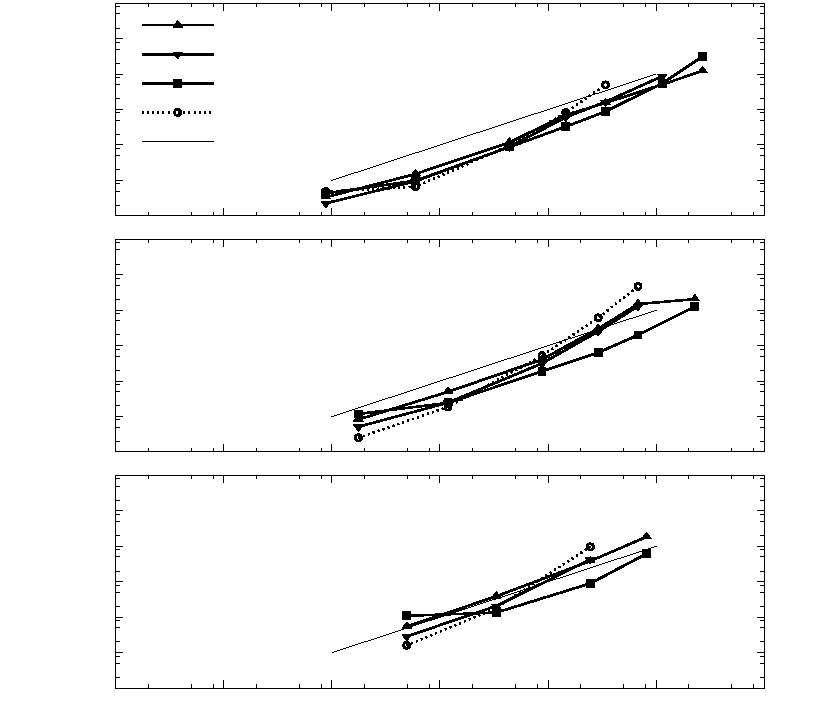
\includegraphics{XdgPoissonScaling}}%
    \gplfronttext
  \end{picture}%
\endgroup
